%%%%%%%%%%%%%%%%%%%%%%%%%%%%%%%%%%%%%%%%%%%%%%%%%%%%%%%%%%%%%%%%%%%%%%%%%
\section{Statistical Properties}  %%%%%%%%%%%%%%%%%%%%%%%%%%%%%%%%%%%%%%%
\label{cr:sec:theory}

In this section, we describe some important statistical properties of the network choice model.
We begin by observing that $\BigO{n}$ values summarizing the traffic at each node is a sufficient statistic for the $\BigO{n^2}$ entries of the Markov-chain transition matrix.
We then connect our statistical model to the steady-state inversion problem defined by \citet{kumar2015inverting}.
Guided by this connection, we study the maximum-likelihood (ML) estimate of model parameters, but find that the estimate is likely to be ill-defined in many scenarios of practical interest.
Lastly, we study how to overcome this issue by introducing a prior distribution on the parameters $\bm{\lambda}$; the prior guarantees that the inference problem is well-posed.

For simplicity of exposition, we present our results for Luce's standard choice model defined in~\eqref{cr:eq:singlelik}.
Our developments extend to the model variant proposed by \citet{kumar2015inverting}, where choice probabilities can be modulated by edge weights.
In Appendix~\ref{cr:app:extensions}, we describe this variant and give the necessary adjustments to our developments.

%%%%%%%%%%%%%%%%%%%%%%%%%%%%%%%%%%%%%%%%%%%%%%%%%%%%%%%%%%%%%%%%%%%%%%%%%
\subsection{Sufficient Statistic}

Let $c_{ij}$ denote the number of transitions that occurred along edge $(i, j) \in E$.
Starting from the transition probability defined in~\eqref{cr:eq:singlelik}, we can write the log-likelihood of $\bm{\lambda}$ given data $\mathcal{D} = \{ c_{ij} \mid (i, j) \in E \}$ as
\begin{align}
\ell(\bm{\lambda} ; \mathcal{D})
    &= \sum_{(i,j) \in E} c_{ij} \bigg[ \log \lambda_j - \log \sum_{k \in N^+_i} \lambda_k \bigg] \nonumber \\
    &= \sum_{j = 1}^n \sum_{i \in N^-_j}\!c_{ij} \log \lambda_j
       - \sum_{i = 1}^n \sum_{j \in N^+_i}\!c_{ij} \log \sum_{k \in N^+_i} \lambda_k \nonumber \\
    &= \sum_{i = 1}^n \bigg[ c^-_i \log \lambda_i - c^+_i \log \sum_{k \in N^+_i} \lambda_k \bigg], \label{cr:eq:loglik}
\end{align}
where $c^-_i = \sum_{j \in N^-_i} c_{ji}$ and $c^+_i = \sum_{j \in N^+_i} c_{ij}$ is the aggregate number of transitions arriving in and originating from $i$, respectively.
This formulation of the log-likelihood exhibits a key feature of the model:
the set of $2n$ counts $\{ (c^-_i, c^+_i) \mid i \in V \}$ is a sufficient statistic of the $\BigO{n^2}$ counts $\{ c_{ij} \mid (i, j) \in E \}$ for the parameters $\bm{\lambda}$.
(In Appendix~\ref{cr:app:extensions}, we show that it is in fact minimally sufficient.)
In other words, it is enough to observe marginal information about the number of arrivals and departures at each node---we collectively call this data the \emph{traffic} at a node---and no additional information can be gained by observing the full choice process.
This makes the model particularly attractive, because it means that it is unnecessary to track users across nodes.
In several applications of practical interest, tracking users is undesirable, difficult, or outright impossible, due to
\begin{enuminline}
\item privacy reasons,
\item monitoring costs, or
\item lack of data in existing datasets.
\end{enuminline}

Note that if we make the additional assumption that the flow in the network is conserved, then $c^-_i = c^+_i$.
If users' typical trajectories consist of many hops, it is reasonable to approximate $c^-_i$ or $c^+_i$ using that assumption, should one of the two quantities be missing.

%%%%%%%%%%%%%%%%%%%%%%%%%%%%%%%%%%%%%%%%%%%%%%%%%%%%%%%%%%%%%%%%%%%%%%%%%
\subsection{Connection to the Steady-State Inversion Problem}
% Also works if all the Markov trajectories are loops.

In recent work, \citet{kumar2015inverting} define the problem of \emph{steady-state inversion} as follows:
Given a strongly-connected directed graph $G = (V, E)$ and a target distribution over the nodes $\bm{\pi}$, find a Markov chain on $G$ with stationary distribution $\bm{\pi}$.
As there are $m = \BigO{n^2}$ degrees of freedom (the transition probabilities) for $n$ constraints (the stationary distribution), the problem is in most cases underdetermined.
Following Luce's ideas, the transition probabilities are constrained to be proportional to a latent score of the destination node as per \eqref{cr:eq:singlelik}, thus reducing the number of parameters from $m$ to $n$.
Denote by $P(\bm{s})$ the Markov-chain transition matrix parametrized with scores $\bm{s}$.
The score vector $\bm{s}$ is a solution for the steady-state inversion problem if and only if $\bm{\pi} = \bm{\pi} P(\bm{s})$, or equivalently
\begin{align}
\label{cr:eq:balance}
\pi_i = \sum_{j \in N^-_i} \frac{s_i}{\sum_{k \in N^+_j} s_k} \pi_j \quad \forall i.
\end{align}
In order to formalize the connection between \citeauthor{kumar2015inverting}'s work and ours, we now express the steady-state inversion problem as that of asymptotic maximum-likelihood estimation in the network choice model.
Suppose that we observe node-level traffic data $\mathcal{D} = \{ (c^-_i, c^+_i) \mid i \in V \}$ about a trajectory of length $T$ starting at an arbitrary node.
We want to obtain an estimate of the parameters $\bm{\lambda}^\star$ by maximizing the average log-likelihood $\hat{\ell}(\bm{\lambda}) = \frac{1}{T} \ell (\bm{\lambda} ; \mathcal{D})$.
From standard convergence results for Markov chains \citep{kemeny1976finite}, it follows that as $G$ is strongly connected, $\lim_{T \to \infty} c^-_i / T = \lim_{T \to \infty} c^+_i / T = \pi_i$.
Therefore,
\begin{align*}
\hat{\ell}(\bm{\lambda})
    = \sum_{i = 1}^n \bigg[ \frac{c^-_i}{T} \log \lambda_i - \frac{c^+_i}{T} \log \sum_{k \in N^+_i} \lambda_k \bigg]
    \xrightarrow{T \to \infty} \sum_{i = 1}^n \pi_i \bigg[ \log \lambda_i - \log \sum_{k \in N^+_i} \lambda_k \bigg].
\end{align*}
Let $\bm{\lambda}^\star$ be a maximizer of the average log-likelihood.
When $T \to \infty$, the optimality condition $\nabla \hat{\ell} (\bm{\lambda}^\star) = \bm{0}$ implies
\begin{align}
\frac{\partial \hat{\ell}(\bm{\lambda})}{\partial \lambda_i} \bigg|_{\bm{\lambda} = \bm{\lambda}^\star}
    = \frac{\pi_i}{\lambda^\star_i} - \sum_{j \in N^-_i} \frac{\pi_j}{\sum_{k \in N^+_j} \lambda^\star_k} = 0
    \iff \pi_i &= \sum_{j \in N^-_i} \frac{\lambda^\star_i}{\sum_{k \in N^+_j} \lambda^\star_k} \pi_j \quad \forall i. \label{cr:eq:optimality}
\end{align}
Comparing~\eqref{cr:eq:optimality} to~\eqref{cr:eq:balance}, it is clear that $\bm{\lambda}^\star$ is a solution of the steady-state inversion problem.
As such, the network choice model presented in this chapter can be viewed as a principled extension of the steady-state inversion problem to the finite-data case.


%%%%%%%%%%%%%%%%%%%%%%%%%%%%%%%%%%%%%%%%%%%%%%%%%%%%%%%%%%%%%%%%%%%%%%%%%
\subsection{Maximum-Likelihood Estimate}
\label{cr:sec:maxlik}

The log-likelihood~\eqref{cr:eq:loglik} is not concave in $\bm{\lambda}$, but it can be made concave using the simple reparametrization $\lambda_i = e^{\theta_i}$.
Therefore, any local minimum of the likelihood is a global minimum.
Unfortunately, it turns out that the conditions guaranteeing that the ML estimate is well-defined (i.e., that it exists and is unique) are restrictive and impractical.
We illustrate this by providing a necessary condition, and for brevity we defer the comprehensive analysis of the ML estimate to Appendix~\ref{cr:app:maxlik}.
We begin with a definition that uses the notion of \emph{hypergraph}, a generalized graph where edges may be any non-empty subset of nodes.
\begin{definition}[comparison hypergraph]
Given a directed graph $G = (V, E)$, the \emph{comparison hypergraph} is the hypergraph $H = (V, \mathcal{A})$, with $\mathcal{A} = \{ N^+_i \mid i \in V \}$.
\end{definition}
Intuitively, $H$ is the hypergraph induced by the sets of alternatives available at each node.
Figure~\ref{cr:fig:samplehyp} provides an example of a graph and of its associated comparison hypergraph.
Equipped with this definition, we can state the following theorem that is a reformulation of a well-known result for Luce's choice model \citep{hunter2004mm}.
\begin{theorem}
\label{cr:thm:mlnecessary}
If the comparison hypergraph is not connected, then for any data $\mathcal{D}$ there are $\bm{\lambda}$ and $\bm{\mu}$ such that $\bm{\lambda} \neq c \bm{\mu}$ for any $c \in \mathbf{R}_{>0}$ and $\ell(\bm{\lambda} ; \mathcal{D}) = \ell(\bm{\mu} ; \mathcal{D}).$
\end{theorem}
In short, the proof shows that rescaling all the parameters in one of the connected components does not change the value of the likelihood function.
The network of Figure~\ref{cr:fig:samplenet} illustrates an instance where the condition fails:
although the graph $G$ is strongly connected, its associated comparison hypergraph $H$ (depicted in Figure~\ref{cr:fig:samplehyp}) is disconnected, and no matter what the data $\mathcal{D}$ is, the ML estimate will never be uniquely defined.
In fact, in Appendix~\ref{cr:app:maxlik}, we demonstrate that Theorem~\ref{cr:thm:mlnecessary} is just the tip of the iceberg.
We provide an example where the ML estimate \emph{does not exist} even though the comparison hypergraph is connected, and we explain that verifying a necessary and sufficient condition for the existence of the ML estimate is computationally \emph{more expensive} than solving the inference problem itself.
%All in all, these shortcomings drive us to seek a more robust estimator.

\begin{figure}[t]
  \centering
  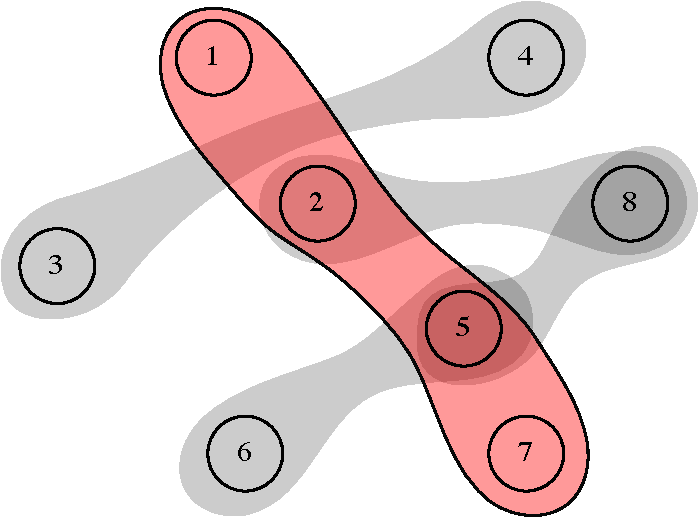
\includegraphics[width=.5\linewidth]{cr-graph-example-pref}
  \caption{The comparison hypergraph associated to the network of Fig.~\ref{cr:fig:samplenet}.
The hyperedge associated to $N^+_6$ is highlighted in red.
Note that the component $\{3, 4\}$ is disconnected from the rest of the hypergraph.}
  \label{cr:fig:samplehyp}
\end{figure}


%%%%%%%%%%%%%%%%%%%%%%%%%%%%%%%%%%%%%%%%%%%%%%%%%%%%%%%%%%%%%%%%%%%%%%%%%
\subsection{Well-Posed Inference}
% https://en.wikipedia.org/wiki/Well-posed_problem

Following the ideas of \citet{caron2012efficient}, we introduce an independent Gamma prior on each parameter, i.e., i.i.d. $\lambda_1, \ldots, \lambda_n \sim \text{Gamma}(\alpha, \beta)$.
Adding the log-prior to the log-likelihood, we can write the log-posterior as
\begin{align}
\begin{aligned}
\label{cr:eq:logpost}
\log p(\bm{\lambda} \mid \mathcal{D}) = \sum_{i = 1}^n
  \bigg[ (c^-_i + \alpha - 1) \log \lambda_i
        - c^+_i \log\!\sum_{k \in N^+_i}\!\lambda_k  - \beta \lambda_i \bigg] + \kappa,
\end{aligned}
\end{align}
where $\kappa$ is a constant that is independent of $\bm{\lambda}$.
The Gamma prior translates into a form of regularization that makes the inference problem well-posed, as shown by the following theorem.

\begin{theorem}
\label{cr:thm:map}
If i.i.d. $\lambda_1, \ldots, \lambda_n \sim \text{Gamma}(\alpha, \beta)$ with $\alpha > 1$, then the log-posterior~\eqref{cr:eq:logpost} always has a unique maximizer $\bm{\lambda}^\star \in \mathbf{R}^n_{>0}$.
\end{theorem}

The condition $\alpha > 1$ ensures that the prior has a nonzero mode.
In short, the proof of Theorem~\ref{cr:thm:map} shows that as a result of the Gamma prior, the log-posterior can be reparametrized into a strictly concave function with bounded super-level sets (if $\alpha > 1$).
This guarantees that the log-posterior will always have exactly one maximizer.
Unlike the results that we derive for the ML estimate, Theorem~\ref{cr:thm:map} does not impose any condition on the graph $G$ for the estimate to be well-defined.

\paragraph{Remark}
Note that varying the rate $\beta$ in the Gamma prior simply rescales the parameters $\bm{\lambda}$.
Furthermore, it is clear from~\eqref{cr:eq:singlelik} that such a rescaling affects neither the likelihood of the observed data nor the prediction of future transitions.
As a consequence, we may assume that $\beta = 1$ without loss of generality.
